\documentclass{article}

\usepackage{cite}
\usepackage[final]{style}
\usepackage[utf8]{inputenc} % allow utf-8 input
\usepackage[T1]{fontenc}    % use 8-bit T1 fonts
\usepackage{hyperref}       % hyperlinks
\usepackage{url}            % simple URL typesetting
\usepackage{booktabs}       % professional-quality tables
\usepackage{amsfonts}       % blackboard math symbols
\usepackage{nicefrac}       % compact symbols for 1/2, etc.
\usepackage{microtype}      % microtypography
\usepackage{verbatim}
\usepackage{graphicx}       % for figures
\usepackage{amsmath}   		% for vectors, matrices
\newcommand{\norm}[1]{\left\lVert #1 \right\rVert} % for latex newbies, I'm defining the norm
% brackets as a math command so that I can refer to it later as just \norm{...} and it will
% autopopulate the nice double brackets
\newcommand*{\vertbar}{\rule[-1ex]{0.5pt}{2.5ex}} % for complicated matrices
\newcommand*{\horzbar}{\rule[.5ex]{2.5ex}{0.5pt}}

\title{Lecture \#2: Color and Linear Algebra pt.1}

\author{
  John McNelly, Alexander Haigh, Madeline Saviano, Scott Kazmierowicz, Cameron Van de Graaf \\
  Department of Computer Science\\
  Stanford University\\
  Stanford, CA 94305 \\
  \texttt{\{jmcnelly, haighal, msaviano, scottkaz, camvdg\}@cs.stanford.edu} \\
}

\begin{document}

\maketitle

\section{Physics of Color}
\subsection{What is color?}
Color is the result of interaction between physical light in the environment and our visual system.  A psychological property of our visual experiences when we look at objects and lights, not a physical property of those objects or lights.  ~\cite{palmer1999vision}


\subsection{Color and light}
White light is composed of almost equal energy in all wavelengths of the visible spectrum

\subsection{Electromagnetic Spectrum}
Light is made up of waves of different wavelengths.  The visual spectrum of light ranges from 400nm to 700nm, and humans are most sensitive to light with wavelengths in the middle of this spectrum.  Humans see only visible light because the Sun emits yellow light more than any other color and due to its temperature.

\subsection{Visible light}
Plank's Law for Blackbody radiation estimates the wavelengths of electromagnetic radiation emitted by a star, based on surface temperature.  For instance, since the surface of the sun is around 5800K, the peak of the sun's emitted light lies in the visible region.

\subsection{The Physics of Light}
Any source of light can be completely described physically by its spectrum (i.e., the amount of energy emitted, per time unit, at each wavelength 400-700nm).  Surfaces have reflectance spectra: reflected light is focused on a certain side of the visible light spectrum. For example, bananas reflect mostly yellow light, and tomatoes reflect mostly red light.

\subsection{Interaction of light and surfaces}
Reflected color is the result of interaction of the light source spectrum with the surface reflectance.  As a rule, definitions and units are stated as "per unit wavelengths", and terms are assumed to be "spectral" (i.e., referring to a spectrum of light, not a single wavelength).  Illumination is quantified as $Illumination .* Reflectance = Color Signal$ ~\cite{wandell1995foundations}

\section{Human Encoding of Color}
As mentioned in the previous section, color is not a mere physical property of light - rather, the phenomenon of color arises via the interaction between light and the human visual system.
\subsection{Rods and Cones}
When we look at a scene, light first enters our eyes through the pupil before reaching the retina. The retina is primarily composed of two types of light-sensitive cells: rods and cones, named for their appearance under a microscope. \textbf{Rods} are the more numerous of the two and are highly sensitive, making them ideal for detecting objects in low-light conditions. However, they do not encode any color information. \textbf{Cones}, on the other hand, are less numerous and less sensitive, but they are useful for distinguishing between objects in high light conditions. They also allow us to perceive colors by a mechanism discussed below.

\subsection{Cones and Color}
A crucial difference between rods and cones is that the latter comes in three different types, each characterized by a unique response curve to different wavelengths of light. Each response curve peaks at a unique wavelength, namely 440, 530, and 560nm, aligning with the colors of blue, green, and red. However, both cones and rods act as \textbf{filters}, the output of which can be interpreted as the multiplication of each response curve by the spectrum, integrated over all wavelengths. While the information encoded by the resulting three numbers is sufficient for most tasks, some information is lost in the compression from spectrum to electrical impulse in the retina. This implies that some subset(s) of spectra will be erroneously perceived as identical - such spectra are called \textbf{metamers}

\subsection{Color Matching}
Since we are interested in designing systems that provide a consistent visual experience across viewers, it is helpful to understand the minimal colors that can be combined to create the experience of any perceivable color. An experiment from Wandell's Foundations of Vision (Sinauer Assoc., 1995) demonstrates that most people report being able to recreate the color of a given test light by tuning three experimental lights of differing colors. The only condition is that each of three lights must be a primary color. Moreover, the experiment showed that for the same test light and primaries,	the majority of people select similar weights, though color blind people are an exception. Finally, this experiment validates the trichromatic theory of color - the proposition that three	numbers	are	sufficient	for	encoding color -  which dates from Thomas Young's writings in the 1700s.


\section{Color Spaces}
\subsection{Definition}
Color space, also known as the color model (or color system), is an abstract mathematical model which describes the range of colors as tuples of numbers, typically as 3 or 4 values or color components (e.g. RGB). A color space may be arbitrary or structured mathematically. Most color models map to an absolute and globally understood system of color interpretation.

\subsection{Linear Color Spaces}
	Defined by a choice of three primaries, and the coordinates of the color are given by the weights of the primaries used to match it

    \begin{figure}[h!]
    \centering
    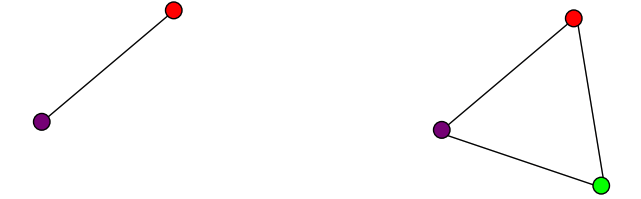
\includegraphics[width=10cm]{color1.png}
    \caption{Mixing two lights produces colors that lie along a straight line in color space. Mixing three lights produces colors that lie within the triangle they define in color space.}
    \end{figure}

    \begin{itemize}
    \item RGB Space
     \begin{itemize}
     \item Primary colors are monochromatic lights (for monitors, they correspond to the three types of phosphors)
     \item Subtractive matching is required for certain wavelengths of light

	  \begin{figure}[h!]
      \centering
      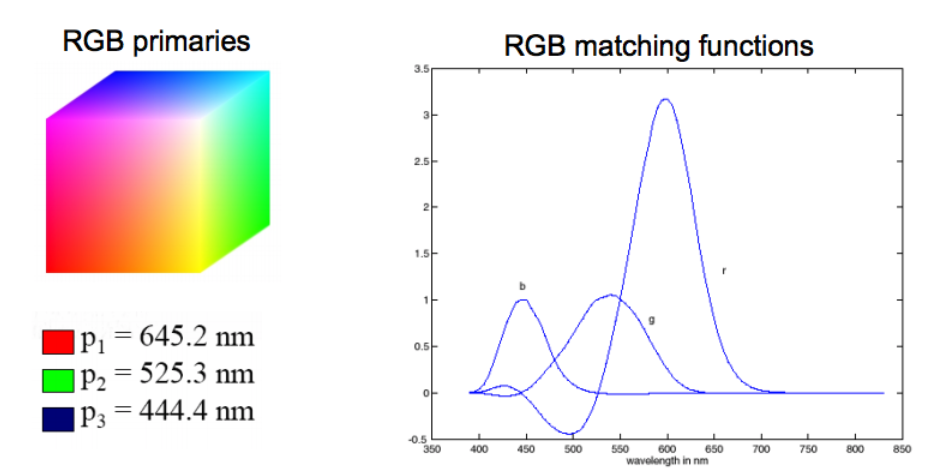
\includegraphics[width=10cm]{rgb1.png}
      \caption{Representation of RBG primaries and corresponding matching functions. The matching functions are the amounts of primaries needed to match the monochromatic test color at the wavelength shown on the horizontal scale. Source: \url{https://en.wikipedia.org/wiki/CIE_1931_color_space}}
      \end{figure}

     \end{itemize}

    \item CIE XYZ Color Space
     \begin{itemize}
     \item Primaries are imaginary, but matching functions are everywhere positive
     \item The Y parameter corresponds to brightness or luminance of a color
     \item Related to RGB space by linear transformation, upholding Grassmann's Law

	  \begin{figure}[h!]
      \centering
      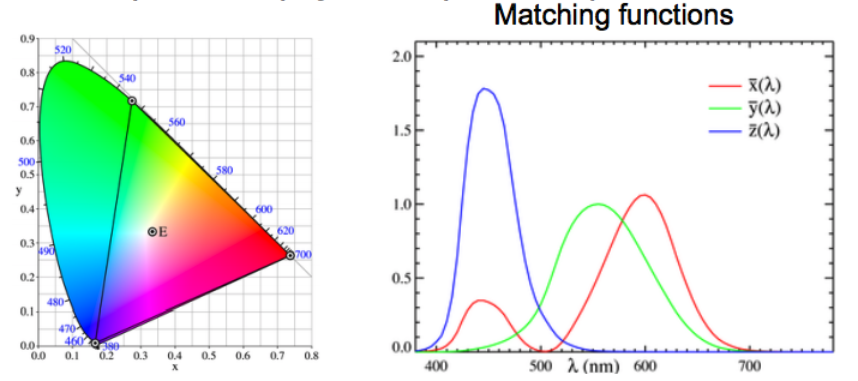
\includegraphics[width=10cm]{xyz1.png}
      \caption{Source: \url{https://en.wikipedia.org/wiki/CIE_1931_color_space}}
      \end{figure}

     \end{itemize}
    \end{itemize}

\subsection{Nonlinear Color Spaces: HSV}
    \begin{itemize}
	\item Designed to reflect more traditional and intuitive color mixing models (e.g. paint mixing)
    \item Based on how colors are organized and conceptualized in human vision
    \item Dimensions are: Hue, Saturation, and Value (Intensity)

\end{itemize}

    \begin{figure}[h!]
    \centering
    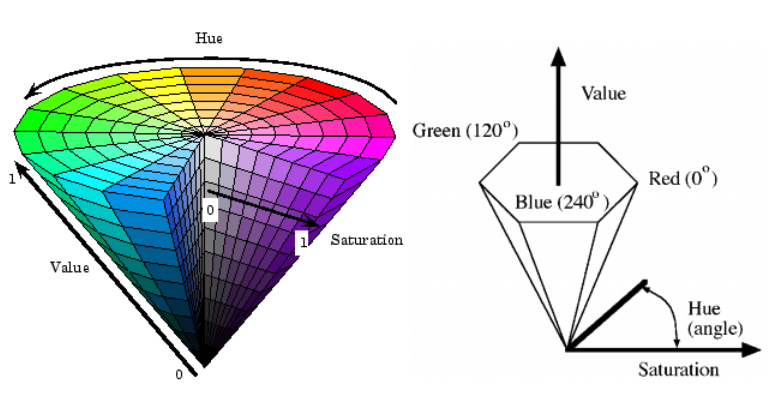
\includegraphics[width=10cm]{hsv1.png}
    \caption{General source: \url{https://en.wikipedia.org/wiki/HSL_and_HSV}}
    \end{figure}


\section{White Balancing}

\subsection{Definition} White Balance is the processing of adjusting the image data received by sensors to properly render neutral colors (white, gray, etc).  This adjustment is performed automatically by digital cameras (custom settings for different light), and film cameras offer several filters and film types for different shooting conditions.

\subsection{Importance of White Balancing} Unadjusted images have an unnatural color "cast" for a few reasons, making white balancing very important:
\begin{enumerate}
\item The sensors in cameras or film are different from those in our eyes
\item Different display media render images differently, which must be accounted for
\item The viewing conditions when the image was taken are usually different from the image viewing conditions
\end{enumerate}

\begin{figure}[h!]
\centering
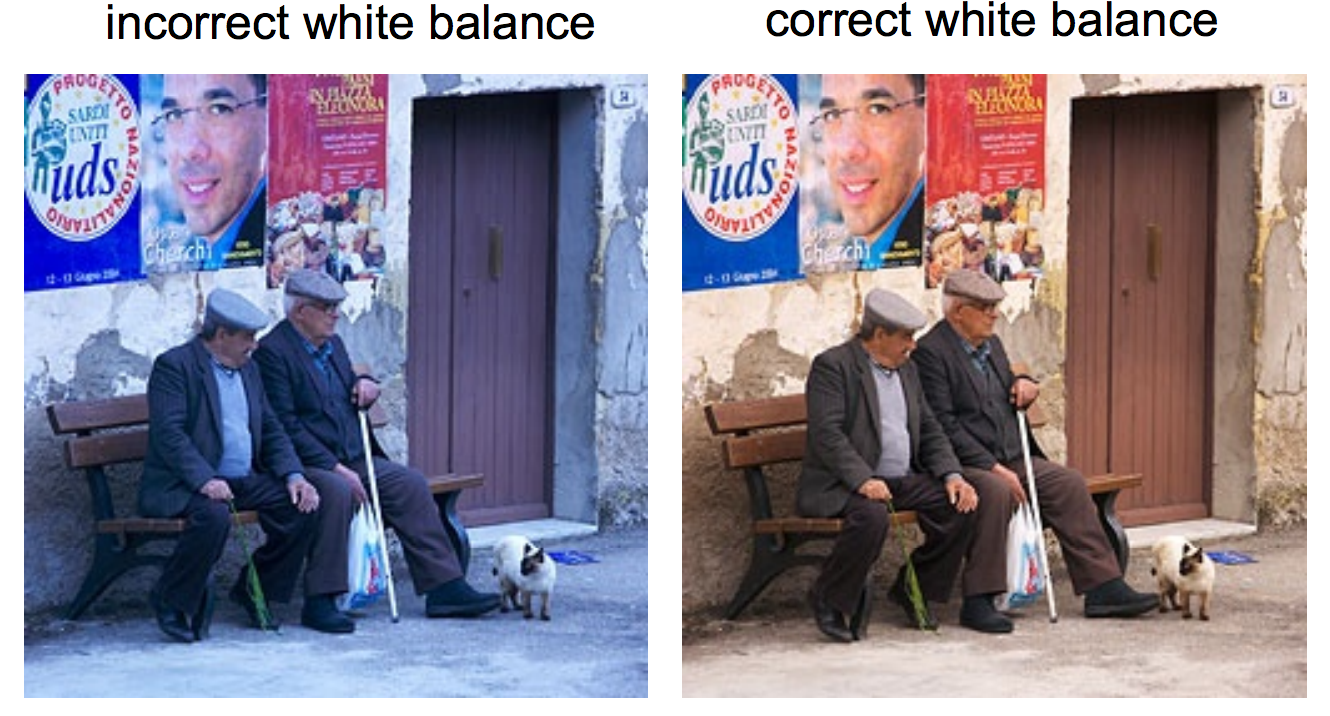
\includegraphics[width=10cm]{wb.png}
\caption{Example of two photos, one unbalanced, and one with incorrect white balancing.  Source: \url{http://www.cambridgeincolour.com/tutorials/white-balance.htme}}
\end{figure}


**Upload images from slides
\subsection{Von Kries Method}
Von Kries' method for white balancing was to scale each channel by a "gain factor" to match the appearance of a gray neutral object.

In practice, the best way to achieve this is the \textbf{Gray Card Method}: hold up a neutral (gray or white) and determine the values of each channel.  If we find that the card has RGB values $r_w,\ g_w,\ b_w$, then we scale each channel of the image by $\frac{1}{r_w},\ \frac{1}{g_w},\ \frac{1}{b_w}$.

\subsection{Other Methods}
Without Gray Cards, we need to guess which pixels correspond to white objects.  Several methods attempt to achieve this, including statistical and Machine Learning models (which are beyond the scope of this class)

\paragraph{Gray World Assumption} Under this model, we assume that the average pixel value in the photo ($r_{ave},\ g_{ave},\ b_{ave}$) is gray and scale the image pixels by $\frac{1}{r_{ave}},\ \frac{1}{g_{ave}},$ and $\frac{1}{b_{ave}}$

\paragraph{Brightest Pixel Assumption} this works on non-saturated images and assumes that image highlights usually have the color of the light source (which is usually white).  So, it corrects white balance by weighting each channel inversely proportional to the values of the brightest pixels

\paragraph{Gamut Mapping} The \href{https://en.wikipedia.org/wiki/Gamut}{Gamut} of an image is the set of all pixel colors displayed in an image (in mathematical terms, this is a "convex hull" and a subset of all possible color combinations).  We can then apply a transformation to the image that maps the gamut of the image to the gamut of a "standard" image under white light.

\subsection{Other Uses of Color in Computer Vision}
Color plays a critical role in skin detection, nude detection, and image segmentation, among other applications.




\section{Linear Algebra Primer: Vectors and Matrices}
\paragraph{Definition} Vectors and matrices are simply collections of ordered numbers that represent something: movements in space, scaling factors, pixel brightness, etc.

\subsection{Vectors}
\paragraph{A column vector} $v\in \mathbb{R}^{nx1}$ where
 $v = \begin{bmatrix}
      	v_{1} \\
        v_{2} \\
        \vdots \\
        v_{n}
       \end{bmatrix}$.
\paragraph{A row vector} $v^{T}\in \mathbb{R}^{1xn}$ where $v^{T} = \begin{bmatrix}
v_{1} & v_{2} & \dots & v_{n} \end{bmatrix}$. $T$ denotes the transpose operation which flips a matrix over its diagonal, switching the row and column indices of the matrix.

As a note, CS 131 will use column vectors as the default. You can transpose vectors in python: for vector $v$, do $v.t$.

\paragraph{Uses of Vectors} There are two main uses of vectors. Firstly, vectors can represent an offset in 2 or 3 dimensional space. In this case, a point is a vector from the origin. Secondly, vectors can represent data (such as pixels, gradients at an image keypoint, etc.). In this use case, the vectors do not have a geometric interpretation but calculations like "distance" can still have value.

\subsection{Matrices}
\paragraph{A matrix} $\textbf{A} \in \mathbb{R}^{mxn}$ is an array of numbers with $m$ rows and $n$ columns:
\[\textbf{A} = \begin{bmatrix}
    a_{11} & a_{12} & a_{13} & \dots  & a_{1n} \\
    a_{21} & a_{22} & a_{23} & \dots  & a_{2n} \\
    \vdots & \vdots & \vdots & \ddots & \vdots \\
    a_{m1} & a_{m2} & a_{m3} & \dots  & a_{mn}
\end{bmatrix}\]
If $m=n$, we say $\textbf{A}$ is square.

\paragraph{An image} is represented in python as a matrix of pixel brightness. The upper left corner of the image is $[y,x]$. \textbf{Grayscale images} have one number per pixel and are stored as an $mxn$ matrix. \textbf{Color images} have 3 numbers per pixel -- red, green, and blue brightness (RGB) and are thus stored as a $mxnx3$ matrix. Multidimensional matrices like these are called \textbf{tensors}.

\subsection{Basic Matrix Operations}
\paragraph{Addition}
$\begin{bmatrix}
    a & b \\
    c & d \\
\end{bmatrix}
+
\begin{bmatrix}
    1 & 2 \\
    3 & 4 \\
\end{bmatrix}
=
\begin{bmatrix}
    a+1 & b+2 \\
    c+3 & d+4 \\
\end{bmatrix}$ \\
You can only add a matrix with matching dimensions or a scalar. \\
$\begin{bmatrix}
    a & b \\
    c & d \\
\end{bmatrix}
+
7
=
\begin{bmatrix}
    a+7 & b+7 \\
    c+7 & d+7 \\
\end{bmatrix}$
\paragraph{Scaling}
$\begin{bmatrix}
    a & b \\
    c & d \\
\end{bmatrix}
*
3
=
\begin{bmatrix}
    3a & 3b \\
    3c & 3d \\
\end{bmatrix}$
\paragraph{Norm} $\norm{x}_{2} = \sqrt[]{\sum\limits_{i=1}\limits^{n}{x_{i}^{2}}}$ \\
More formally, a norm is any function $f: \mathbf{R}^n \rightarrow \mathbf{R}$ that satisfies four properties:
\begin{enumerate}
  \item \textbf{Non-negativity}: for all $x\in \mathbf{R}^n, f(x) \geq 0$
  \item \textbf{Definiteness}: $f(x) = 0$ if and only if $x=0$
  \item \textbf{Homogeneity}: for all $x\in \mathbf{R}^n, t\in \mathbf{R}, f(tx) = \lvert t\rvert f(x)$
  \item \textbf{Triangle Inequality}: for all $x,y\in \mathbf{R}^n, f(x+y) \leq f(x) + f(y)$
\end{enumerate}
Example Norms:
\paragraph{One Norm} $\norm{x}_{1} = \sum\limits_{i=1}\limits^{n}{\lvert x_{i}\rvert}$
\paragraph{Infinity Norm} $\norm{x}_{\inf} = \textnormal{max}_{i} \lvert x_{i}\rvert$
\paragraph{General P Norm} $\norm{x}_{p} = \bigg(\sum\limits_{i=1}\limits^{n}{x_{i}^{p}}\bigg)^{1/p}$
\paragraph{Matrix Norm} $\norm{A}_{F} = \sqrt[]{\sum\limits_{i=1}\limits^{m}\sum\limits_{j=1}\limits^{n}{A_{ij}^2}} = \sqrt[]{tr(A^TA)}$

\paragraph{Inner or Dot Product} Multiply corresponding entries of two vectors and add up the result. $x\cdot y$ is $\norm{x}\norm{y}\cos(\textnormal{the angle between x and y})$. Thus if $y$ is a unit vector then $x \cdot y$ gives the length of $x$ which lies in the direction of $y$.\\
\textbf{One dimensional dot product}:
$x^Ty = x\cdot y = \begin{bmatrix} x_{1} & \dots & x_{n} \end{bmatrix} \begin{bmatrix} y_{1} \\ \vdots \\ y_{n} \end{bmatrix} = \sum_{i=1}^{n}x_{i}y_{i}$ (scalar)

\paragraph{Multiplication} The product of two matrices $A\in \mathbf{R}^{mxn}, B\in \mathbf{R}^{nxp}$ results in $C = AB \in \mathbf{R}^{mxp}$ where $C_{ij} = \sum\limits_{k=1}\limits^{n}{A_{ik}B_{kj}}$.
\[C = AB = \begin{bmatrix}
     \horzbar & a_{1}^{T} & \horzbar \\
     \horzbar & a_{2}^{T} & \horzbar \\
     & \vdots &  \\
    \horzbar & a_{m}^{T} & \horzbar
\end{bmatrix}
\begin{bmatrix}
    \vertbar & \vertbar & \dots & \vertbar \\
    b_{1} & b_{2} &  \dots  & b_{p} \\
    \vertbar & \vertbar & \dots & \vertbar
\end{bmatrix}
=
\begin{bmatrix}
    a_{1}^{T}b_{1} & a_{1}^{T}b_{2} & \dots  & a_{1}^{T}b_{p} \\
    a_{2}^{T}b_{1} & a_{2}^{T}b_{2} &  \dots  & a_{2}^{T}b_{p} \\
    \vdots & \vdots &  \ddots & \vdots \\
    a_{m}^{T}b_{1} & a_{m}^{T}b_{2} &  \dots  & a_{m}^{T}b_{p}
\end{bmatrix}\]
Each entry of the matrix product is made by taking the dot product of the corresponding row in the left matrix, with the corresponding column in the right one.

Matrix multiplication is
\begin{enumerate}
  \item \textbf{Associative}: $(AB)C = A(BC)$
  \item \textbf{Distributive}: $(A+B)C = AC + BC$
  \item \textbf{Not Commutative}: Generally $AB \neq BA$. For example, if $A\in \mathbb{R}^{mxn}, B \in \mathbb{R}^{nxq}$, the product $BA$ does not even exist if $m$ and $q$ are not equal!
\end{enumerate}

\paragraph{Powers} By convention, we can refer to the matrix product $AA$ as $A^2$ and $AAA$ as $A^3$, etc. Obviously only square matrices can be multiplied that way.

\paragraph{Transpose} Flip matrix so row 1 becomes column 1:
\[
\begin{bmatrix}
    1 & 2 \\
    3 & 4 \\
    5 & 6
\end{bmatrix}^T
=
\begin{bmatrix}
    1 & 3 & 5\\
    2 & 4 & 6\\
\end{bmatrix}
\]
A useful identity: $(ABC)^T = C^TB^TA^T$.

\paragraph{Determinant} $det(\mathbf{A})$ returns a scalar. It represents the area (or volume) of the parallelogram described by the vectors in the rows of the matrix.\\
For $\mathbf{A} = \begin{bmatrix}
    a & b \\
    c & d \\
\end{bmatrix}$, $det(\mathbf{A}) = ad-bc$\\
\textbf{Properties}:
\begin{itemize}
	\item $det(\mathbf{AB}) = det(\mathbf{BA})$
    \item $det(\mathbf{A}^{-1}) = \frac{1}{det(\mathbf{A})}$
    \item $det(\mathbf{A}^T) = det(\mathbf{A})$
    \item $det(\mathbf{A}) = 0$ if and only if \textbf{A} is singular.
\end{itemize}

\paragraph{Trace} $tr(\mathbf{A})$ is the sum of diagonal elements.
For $\mathbf{A} = \begin{bmatrix}
    1 & 3 \\
    5 & 7 \\
\end{bmatrix}$, $tr(\mathbf{A}) = 1+7 = 8$\\
\textbf{Properties}:
\begin{itemize}
	\item $tr(\mathbf{AB}) = tr(\mathbf{BA})$
    \item $tr(\mathbf{A+B}) = tr(\mathbf{A}) + tr(\mathbf{B})$
\end{itemize}

\paragraph{Special Matrices}
\begin{itemize}
	\item Identity Matrix: a square matrix with 1's along the diagonal and 0's elsewhere. \textbf{I} * another matrix $=$ that matrix. Example identity matrix: $\begin{bmatrix}
    1 & 0 & 0 \\
    0 & 1 & 0 \\
    0 & 0 & 1
\end{bmatrix}$
    \item Diagonal Matrix: a square matrix with numbers along the diagonal and 0's elsewhere. A diagonal * another matrix scales the rows of that matrix. Example diagonal matrix: $\begin{bmatrix}
    3 & 0 & 0 \\
    0 & 5 & 0 \\
    0 & 0 & 2.5
\end{bmatrix}$
    \item Symmetric Matrix: $A^T = A$. Example: $\begin{bmatrix}
    1 & 2 & 5 \\
    2 & 1 & 7 \\
    5 & 7 & 1
\end{bmatrix}$
    \item Skew-symmetric matrix:$A^T = -A$. Example: $\begin{bmatrix}
    0 & -2 & -5 \\
    2 & 0 & -7 \\
    5 & 7 & 0
\end{bmatrix}$
\end{itemize}


% References
\small
\bibliographystyle{plain}
\bibliography{bibliography}
\end{document}


